
\section{Predicción en una RNA}

\begin{frame}
	\frametitle{Elementos de una RNA}


	\begin{center}
		\begin{tikzpicture}[scale=0.7, transform shape, >=Stealth]
			% Estilos de nodos
			\tikzset{
				neuron/.style={circle,fill=black!25,minimum size=22pt,inner sep=0pt},
				input neuron/.style={neuron, fill=green!50},
				output neuron/.style={neuron, fill=red!50, align=center},
				hidden neuron/.style={neuron, fill=blue!50, align=center},
				annot/.style={text width=4em, text centered}
			}
			
			% Dibuja la capa de entrada
			\foreach \name / \y in {1,...,2}
			\node[input neuron] (I-\name) at (0,-\y*2.5) {$x_{\name}$};
			
			% Dibuja la capa oculta
			\foreach \name / \y in {1,...,3}
			\node[hidden neuron] (H-\name) at (5cm,-\y*2.5) {$\sigma$};
			
			% Dibuja la capa de salida
			\node[output neuron,pin={[pin edge={->}]right:$\hat{y}$}, right=of H-2] (O) {$\sigma$};
			
			% Conecta las unidades con pesos
			\foreach \source in {1,...,2} {
				\foreach \dest in {1,...,3} {
					\draw (I-\source) -- (H-\dest) node[midway, above, sloped, pos=0.7, xshift=(\source-1.5)*3pt, yshift=(\dest-2)*3pt] {$w_{\source,\dest}$};
				}
			}
			
			% Conecta la capa oculta a la de salida con pesos
			\foreach \source in {1,...,3} {
				\pgfmathtruncatemacro{\result}{\source}
				\draw (H-\source) -- (O) node[midway, above, sloped, yshift=\source*2pt] {$w_{\result,1}$};
			}
			
			% Etiquetas
			\node[annot,above=of H-1, yshift=0.1cm] {Capa oculta};
			\node[annot,left=of I-1, node distance=3cm] (capa_entrada) {Capa de entrada};
			\node[annot,right=of O, node distance=3cm] {Capa de salida};
			
			% Dibuja el vector columna debajo de la etiqueta "Capa de entrada"
			\node[below=0.5cm of capa_entrada] (vector) {${\vec{\mathbf{X}}} = \begin{bmatrix} x_1 \\ x_2 \\ \vdots \\ x_n \end{bmatrix}$};
			
			% Overlay de elementos
			\only<2->{
				\draw[->] (vector) -- (I-1);
				\draw[->] (vector) -- (I-2);
			}
			\only<3->{
				\foreach \source in {1,...,2} {
					\foreach \dest in {1,...,3} {
						\draw[->,red,thick] (I-\source) -- (H-\dest);
					}
				}
			}
			\only<4->{
				% Flecha del sesgo apuntando de arriba hacia abajo a la neurona
				\node[above=0.5cm of H-2] (Bias) {$b$};
				\draw[->,red,thick] (Bias) -- (H-2);
			}
		\end{tikzpicture}
	\end{center}


\end{frame}


\begin{frame}
	\frametitle{Forward propagation: Realizar la predicción}
	\begin{center}
		\begin{tikzpicture}[scale=0.7, transform shape, >=Stealth]
			% Estilos de nodos
			\tikzset{
				neuron/.style={circle,fill=black!25,minimum size=22pt,inner sep=0pt},
				input neuron/.style={neuron, fill=green!50},
				output neuron/.style={neuron, fill=red!50, align=center},
				hidden neuron/.style={neuron, fill=blue!50, align=center},
				annot/.style={text width=4em, text centered}
			}
			
			% Dibuja la capa de entrada
			\foreach \name / \y in {1,...,2}
			\node[input neuron] (I-\name) at (0,-\y*2.5) {$x_{\name}$};
			
			% Dibuja la capa oculta
			\foreach \name / \y in {1,...,3}
			\node[hidden neuron] (H-\name) at (5cm,-\y*2.5) {$\sigma$};
			
			% Dibuja la capa de salida
			\node[output neuron,pin={[pin edge={->}]right:$\hat{y}$}, right=of H-2] (O) {$\sigma$};
			
			% Conecta las unidades con pesos
			\foreach \source in {1,...,2} {
				\foreach \dest in {1,...,3} {
					\draw (I-\source) -- (H-\dest) node[midway, above, sloped, pos=0.7, xshift=(\source-1.5)*3pt, yshift=(\dest-2)*3pt] {$w_{\source,\dest}$};
				}
			}
			
			% Conecta la capa oculta a la de salida con pesos
			\foreach \source in {1,...,3} {
				\pgfmathtruncatemacro{\result}{\source}
				\draw (H-\source) -- (O) node[midway, above, sloped, yshift=\source*2pt] {$w_{\result,1}$};
			}
			
			% Etiquetas
			\node[annot,above=of H-1, yshift=0.1cm] {Capa oculta};
			\node[annot,left=of I-1, node distance=3cm] (capa_entrada) {Capa de entrada};
			\node[annot,right=of O, node distance=3cm] {Capa de salida};
			
			% Dibuja el vector columna debajo de la etiqueta "Capa de entrada"
			\node[below=0.5cm of capa_entrada] (vector) {${\vec{\mathbf{X}}} = \begin{bmatrix} x_1 \\ x_2 \\ \vdots \\ x_n \end{bmatrix}$};
			
			% Conexiones de vector columna
			\draw[->] (vector) -- (I-1);
			\draw[->] (vector) -- (I-2);
			
			% Sesgo
			\node[above=0.5cm of H-2] (Bias) {$b$};
			\draw[->] (Bias) -- (H-2);
			
			% Flecha "forward"
			% Flecha "Forward" controlada manualmente
			\draw[->, thick] (-1, 1) -- node[above] {Forward} (8, 1);
		\end{tikzpicture}
	\end{center}
	
	
\end{frame}

%------------------------------------------------

\begin{frame}
	\frametitle{Funciones de Activación: Sigmoidal}
	{\Large \textit{Son las que 'prenden o apagan' las neuronas}}
	\vspace{5mm}
	\begin{columns}
		
		% Columna de la izquierda
		\begin{column}{0.5\textwidth} % Ajusta la proporción según necesites
			\vspace{-10mm}
			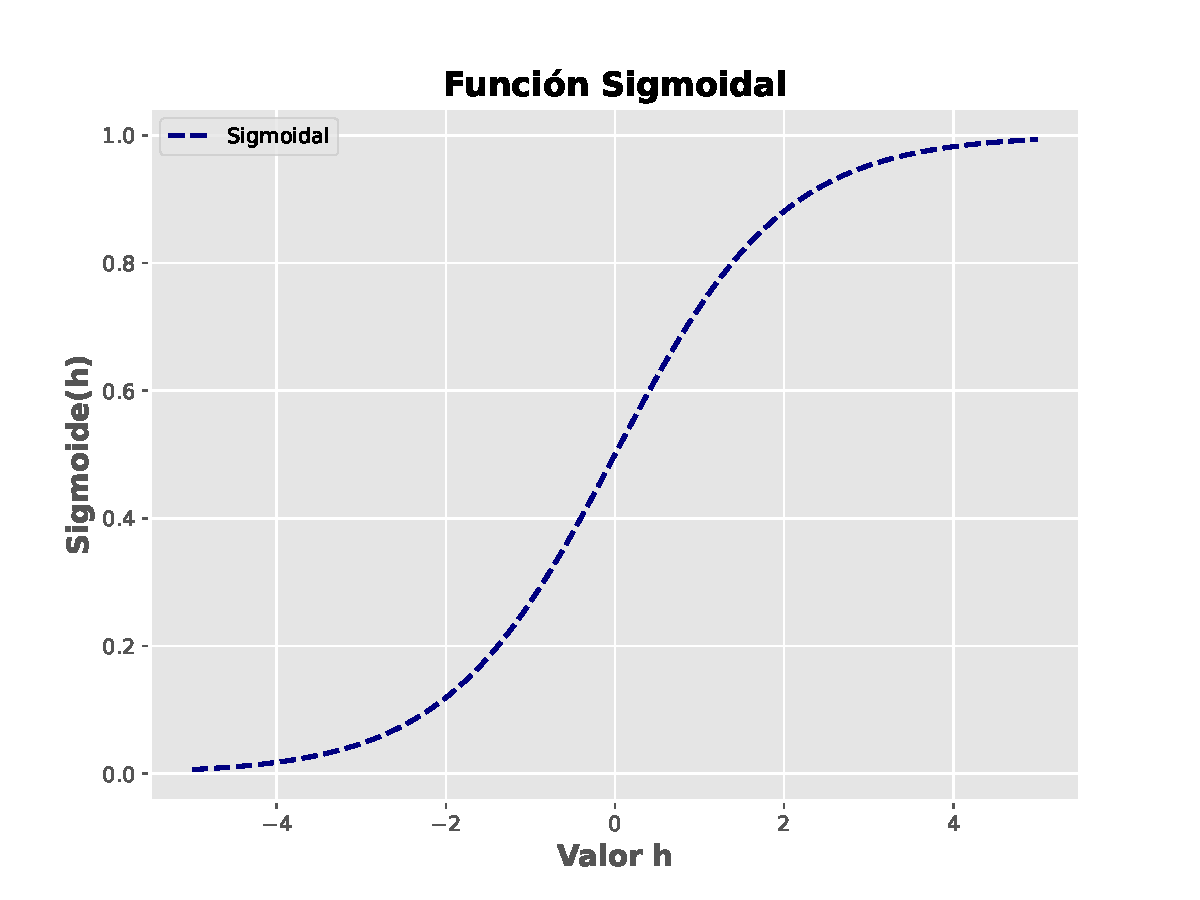
\includegraphics[width=\textwidth]{img/sigmoidal.pdf} % Asegúrate de cambiar la ruta a la ubicación de tu imagen
		\end{column}
		
		% Columna de la derecha
		% Columna de la derecha
		\begin{column}{0.5\textwidth} % Ajusta la proporción según necesites
			\textbf{Expresión matemática:}
			\vspace{-3mm}
			\[ \sigma(x) = \frac{1}{1 + e^{-x}} \]

			\textbf{Dominio y Rango:}
			\begin{itemize}
				\item \textbf{Dominio:} Todos los números reales ($\mathbb{R}$)
				\item \textbf{Rango:} Entre 0 y 1 (0, 1)
			\end{itemize}
			
			\textbf{Descripción:}Mapea cualquier valor real a un valor entre 0 y 1, de ahí su capacidad para interpretar las predicciones como probabilidades.
		\end{column}
		
		
	\end{columns}

\end{frame}

\begin{frame}
	\frametitle{Funciones de Activación: Tanh}
	\begin{columns}
		
		% Columna de la izquierda
		\begin{column}{0.5\textwidth} % Ajusta la proporción según necesites
			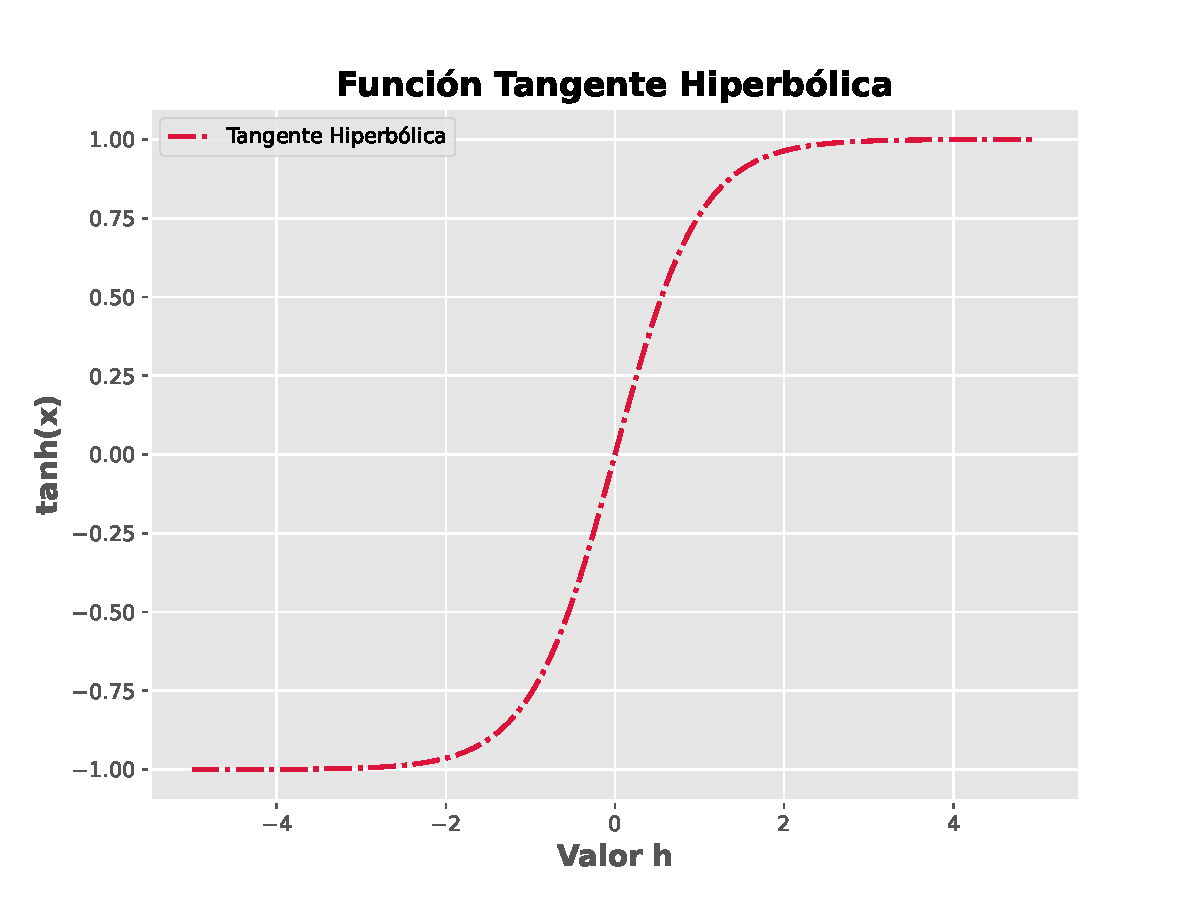
\includegraphics[width=\textwidth]{img/tanh.pdf} % Asegúrate de cambiar la ruta a la ubicación de tu imagen
		\end{column}
		
		% Columna de la derecha
		\begin{column}{0.5\textwidth} % Ajusta la proporción según necesites
			\textbf{Expresión Matemática:}
			\[ \tanh(x) = \frac{e^{x} - e^{-x}}{e^{x} + e^{-x}} \]
			
			\textbf{Dominio y Rango:}
			\begin{itemize}
				\item \textbf{Dominio:} $\mathbb{R}$ 
				\item \textbf{Rango:} $(-1, 1)$
			\end{itemize}
			
			\textbf{Descripción:} Transforma valores en un rango de -1 a 1. Esto la hace útil para modelar decisiones donde una característica aporta un valor positivo/negativo a la predicción.

		\end{column}
		
	\end{columns}
	
\end{frame}


\begin{frame}
	\frametitle{Funciones de Activación: ReLU}
	\begin{columns}
		
		% Columna de la izquierda
		\begin{column}{0.5\textwidth} % Ajusta la proporción según necesites
			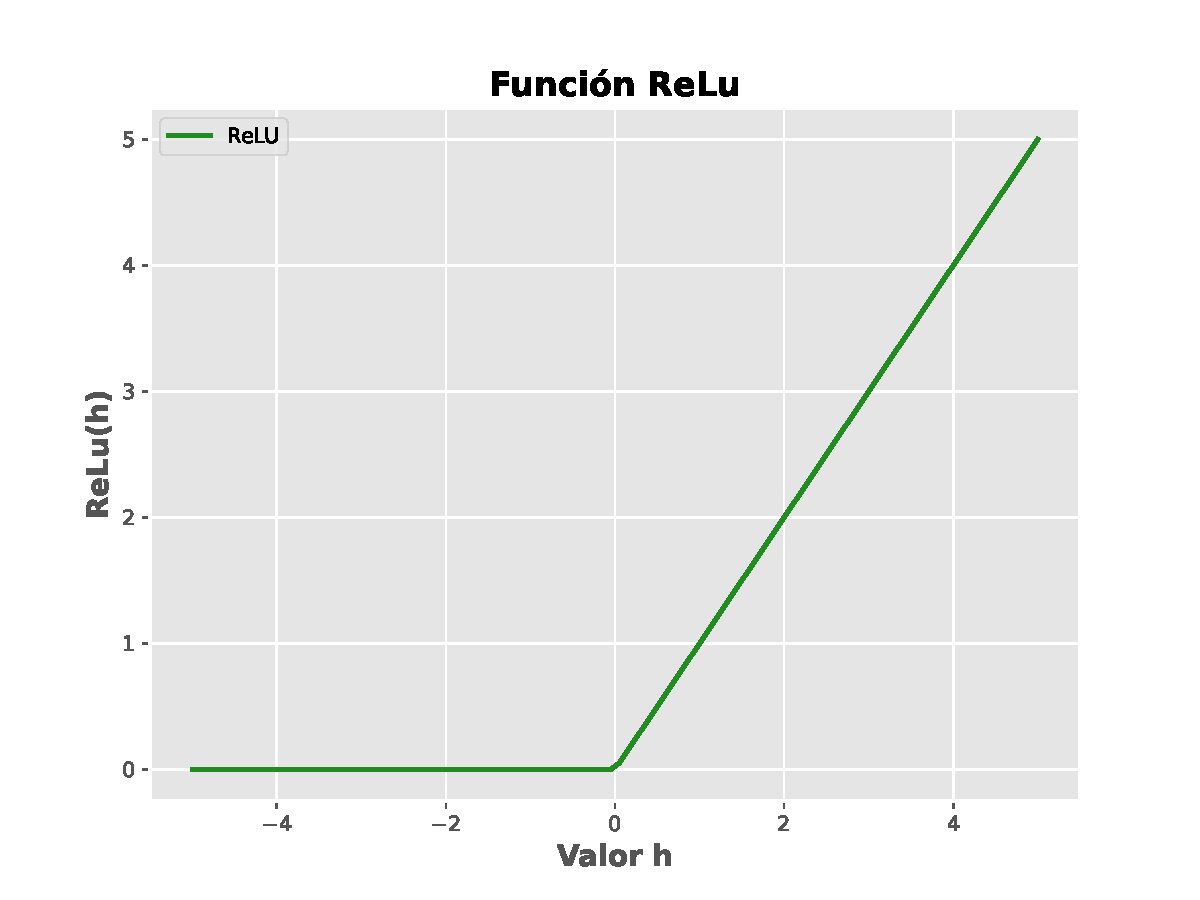
\includegraphics[width=\textwidth]{img/relu.pdf} % Asegúrate de cambiar la ruta a la ubicación de tu imagen
		\end{column}
		
		% Columna de la derecha
		 \begin{column}{0.5\textwidth} % Ajusta la proporción según necesites
			\textbf{Expresión Matemática:}
			\[ \text{ReLU}(x) = \max(0, x) \]
			
			\textbf{Dominio y Rango:}
			\begin{itemize}
				\item \textbf{Dominio:} $\mathbb{R}$ 
				\item \textbf{Rango:} $[0, \infty)$
			\end{itemize}
			
			\textbf{Descripción:} {\normalsize Su simplicidad acelera el proceso de entrenamiento debido a la eficiencia computacional de su cálculo. Además, permite que las neuronas tengan salidas nulas.}
			
			{\normalsize Enfrenta el problema de las neuronas muertas, lo que puede limitar la capacidad de aprendizaje de la red}
		\end{column}
		
	\end{columns}
	
\end{frame}


%------------------------------------------------

